\section{Funcionamiento}
    Se llevaron a cabo diferentes pruebas con estados variados para demostrar la eficiencia de esta alternativa de solución al puzzle, ya que al generar todos los caminos posibles, en muchos casos no tendremos soluciones optivas, lo que causa que las posibilidades sean muy elevadas. La solución para este caso es la siguiente imagen:

    \begin{figure}[!h]
        \centering
        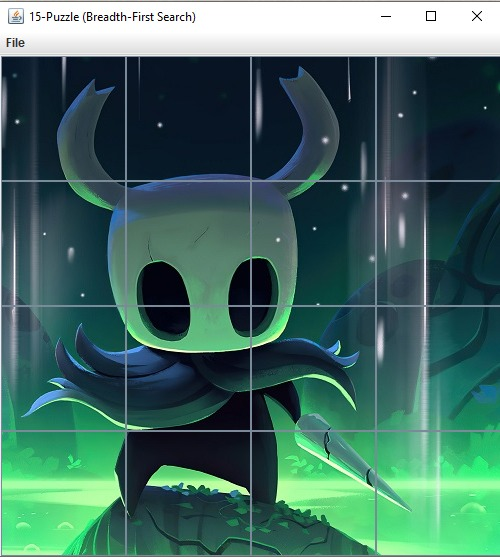
\includegraphics[scale=.4]{Imagenes/final.jpg}
        \caption{Estado final}
        \label{fig:my_label}
    \end{figure}

    \subsection{Prueba 1}
        Se utilizo un caso en donde esta completamente revuelto el puzzle. Y únicamente la bfs pudo encontrar una solución.
        
        \begin{figure}[!h]
          \centering
          \begin{subfigure}{0.3\textwidth}
            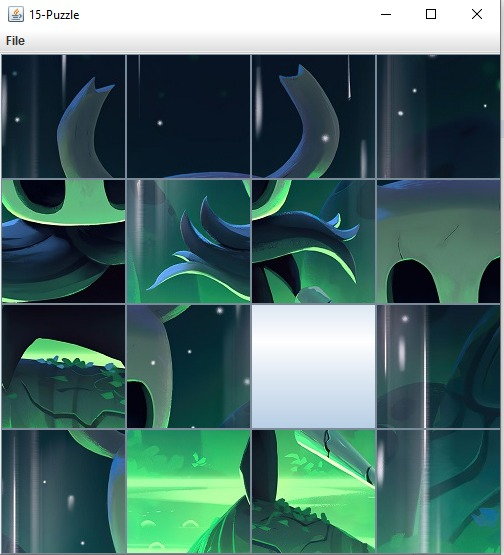
\includegraphics[width=\textwidth]{Imagenes/rev.jpg}
            \caption{Estado inicial}
          \end{subfigure}
          \hfill
          \begin{subfigure}{0.3\textwidth}
            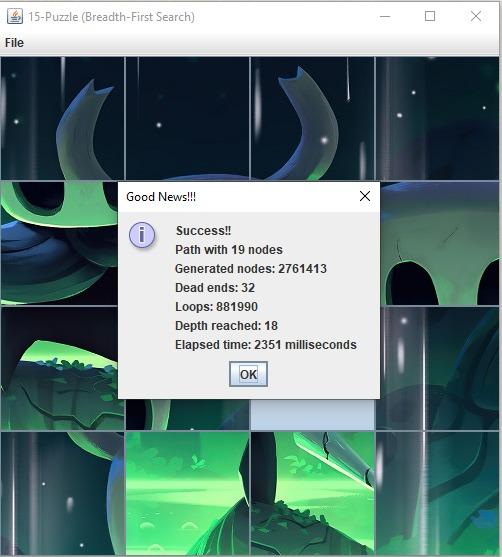
\includegraphics[width=\textwidth]{Imagenes/bfs1.jpg}
            \caption{BFS}
          \end{subfigure}
          \hfill
          \begin{subfigure}{0.3\textwidth}
            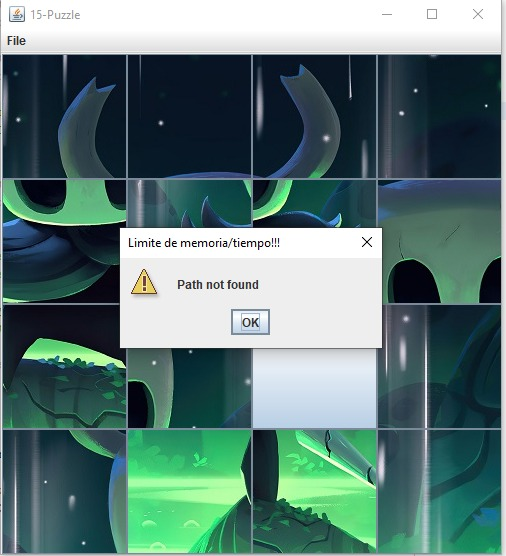
\includegraphics[width=\textwidth]{Imagenes/dfs1.jpg}
            \caption{DFS}
          \end{subfigure}
          \caption{Prueba }
        \end{figure}
        


    
    \subsection{Prueba 2}
        En este caso se muestra un estado casi resuelto, sin embargo, la dfs aún no es capaz de encontrar una solución.

        \begin{figure}[!h]
          \centering
          \begin{subfigure}{0.3\textwidth}
            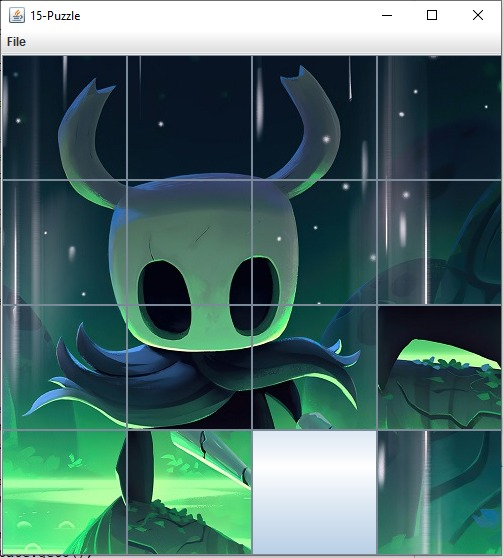
\includegraphics[width=\textwidth]{Imagenes/inicial2.jpg}
            \caption{Estado inicial}
          \end{subfigure}
          \hfill
          \begin{subfigure}{0.3\textwidth}
            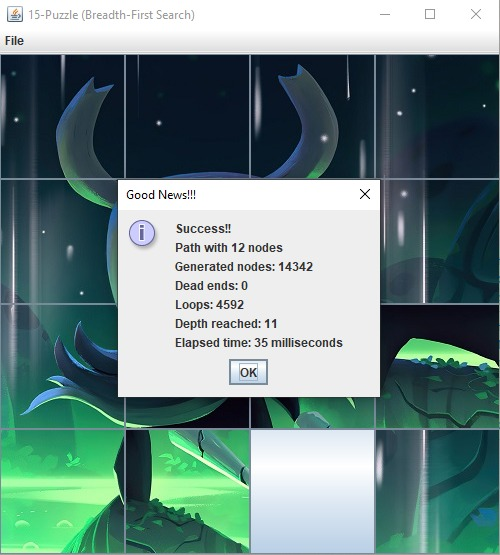
\includegraphics[width=\textwidth]{Imagenes/bfs2.jpg}
            \caption{BFS}
          \end{subfigure}
          \hfill
          \begin{subfigure}{0.3\textwidth}
            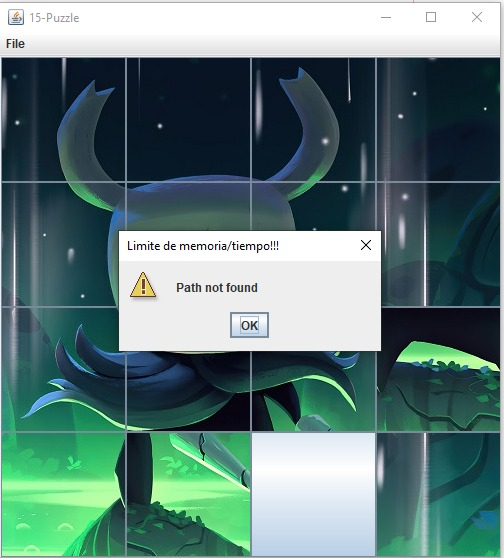
\includegraphics[width=\textwidth]{Imagenes/dfs2.jpg}
            \caption{DFS}
          \end{subfigure}
          \caption{Prueba 2}
        \end{figure}

    \subsection{Prueba 3}
        Después de varias pruebas se llegó a la conclusión que el puzzle debe de estar casi resuelto y con casos planeados para que la dfs pueda funcionar, ya que básicamente este algoritmo explora hasta lo mas profundo de todos cada uno de los estados, por lo que debe de encontrar la solución para cada camino en lugar de ir viendo todos los estados adyacentes de distancia 1 tal y como lo hacer la bfs.
        
        \begin{figure}[!h]
          \centering
          \begin{subfigure}{0.3\textwidth}
            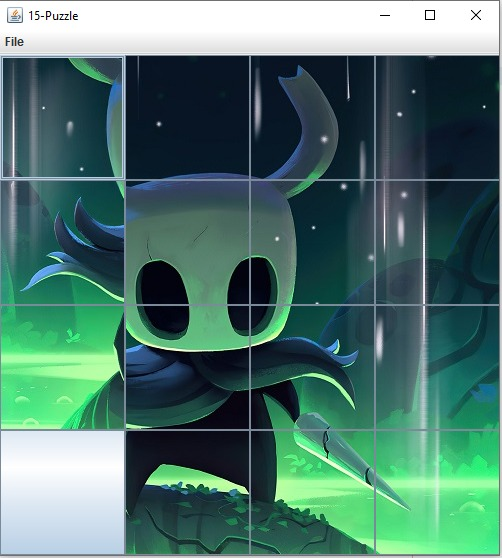
\includegraphics[width=\textwidth]{Imagenes/inicial3.jpg}
            \caption{Estado inicial}
          \end{subfigure}
          \hfill
          \begin{subfigure}{0.3\textwidth}
            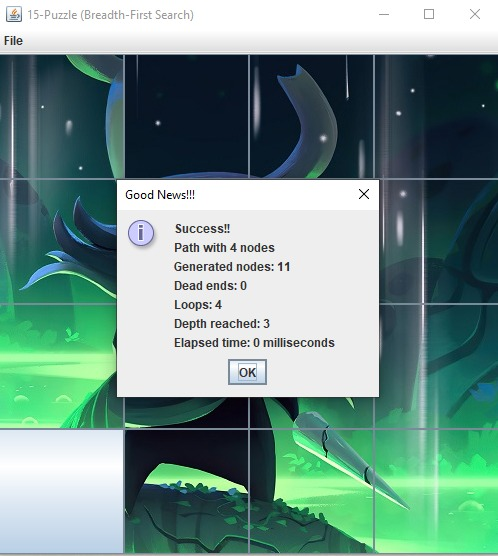
\includegraphics[width=\textwidth]{Imagenes/bfs3.jpg}
            \caption{BFS}
          \end{subfigure}
          \hfill
          \begin{subfigure}{0.3\textwidth}
            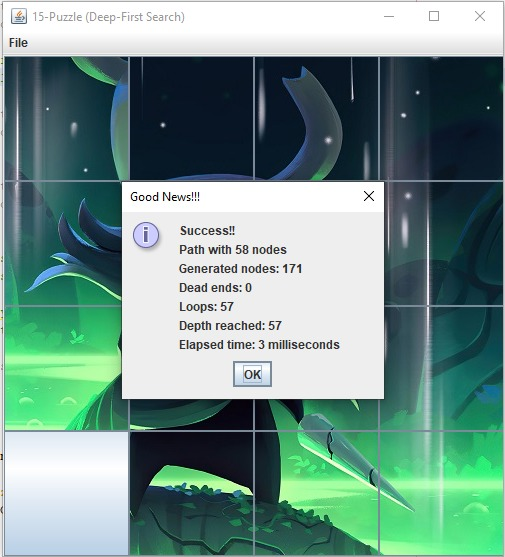
\includegraphics[width=\textwidth]{Imagenes/dfs3.jpg}
            \caption{DFS}
          \end{subfigure}
          \caption{Prueba 3}
        \end{figure}

        Además podemos comprobar que por la naturaleza de la BFS, siempre encontrará el camino más corto, y que la dfs solo devuelve la primera solución encontrada.

\newpage
    
    \subsection{Prueba 4}
        Este caso es interesante, ya que prueba que la cantidad de pizas en sus lugar no determina si es viable encontrar su solución ya que no controlamos los estados adyacentes.
    
        \begin{figure}[!h]
          \centering
          \begin{subfigure}{0.3\textwidth}
            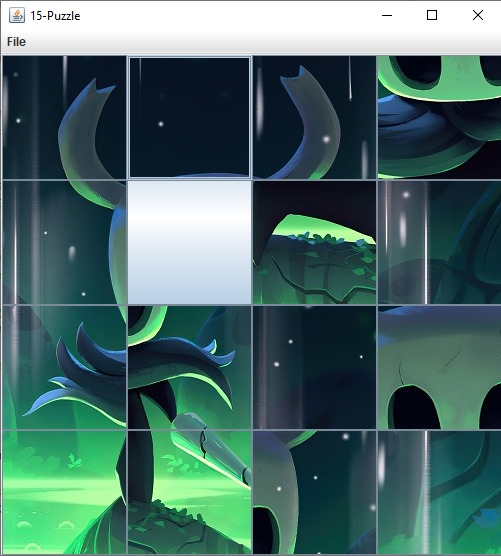
\includegraphics[width=\textwidth]{Imagenes/inicial5.jpg}
            \caption{Estado inicial}
          \end{subfigure}
          \hfill
          \begin{subfigure}{0.3\textwidth}
            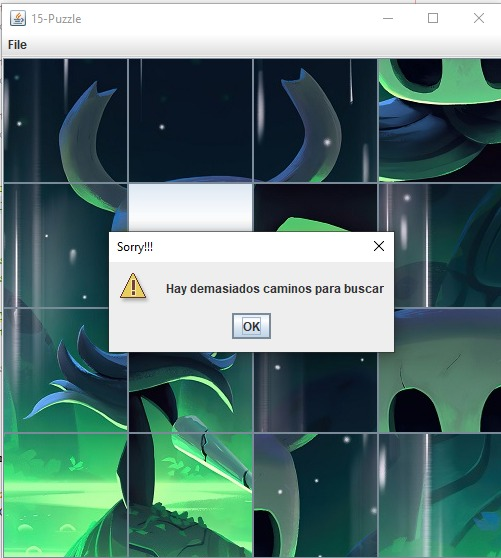
\includegraphics[width=\textwidth]{Imagenes/bfs5.jpg}
            \caption{BFS}
          \end{subfigure}
          \hfill
          \begin{subfigure}{0.3\textwidth}
            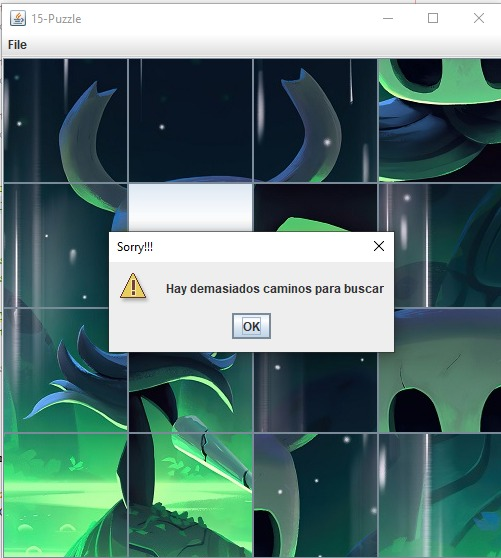
\includegraphics[width=\textwidth]{Imagenes/dfs5.jpg}
            \caption{DFS}
          \end{subfigure}
          \caption{Prueba 4}
        \end{figure}

\section{Conclusiones}
    \begin{itemize}
        \item La BFS siempre encontrara la solución más corta desde la raíz ya que avanza capa por capa o una distancia de 1.
        \item Cuando utilizamos búsquedas no informadas es necesario guardar los estados visitados, pues reduce significativamentes el tiempo de ejecución del programa.
        \item  La DFS no es un algoritmo recomendado si no conocemos el espacio completo de estados, ya que a pesar de que siempre devolverá una solución, esta será la primera en ser encontrada, y no necesariamente la más corta o viable. Es por este que en la mayoría de pruebas se agotó la memoria o excedió las capacidades de la computadora.
        \item La BFS demostró ser más útil cuando buscamos respuestas a ciegas.
    \end{itemize}